\noindent\begin{minipage}{7cm}
\begin{description}
\item[Objectif :] connaître et manipuler les principaux opérateurs booléens.
\item[Syntaxe \python :] \mbox{}
	\begin{itemize}
	\item \texttt{not a}
	\item \texttt{a or b}
	\item \texttt{a and b}
	\item \texttt{a == b}
	\item \texttt{a != b}
	\end{itemize}
\end{description}
\end{minipage}
%\mbox{}\hfill
%\begin{tabular}{c}
%%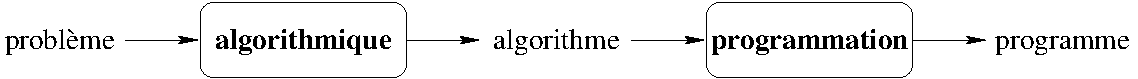
\includegraphics[width=8cm]{informatique-paysage.pdf}
%\end{tabular}

%-------------------------------------------------------------------------
\subsection{Exemple}
%-------------------------------------------------------------------------
\paragraph{Enoncé :}
On considère les conventions graphiques traditionnelles pour les opérateurs 
logiques \texttt{and} ($\cdot$), \texttt{or} ($+$) et \texttt{xor} ($\oplus$) :

\centerline{\begin{tabular}{ccc}
$a \cdot b$ & $a + b$ & $a \oplus b$ \\
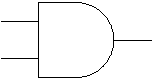
\includegraphics[scale=0.7]{et.pdf} & 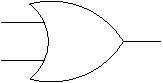
\includegraphics[scale=0.7]{ou.pdf} & 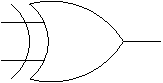
\includegraphics[scale=0.7]{xor.pdf}
\end{tabular}}

On cherche à établir la table de vérité du circuit logique ci-dessous où $a$, $b$
et $c$ sont les entrées, $s$ et $t$ les sorties.
$$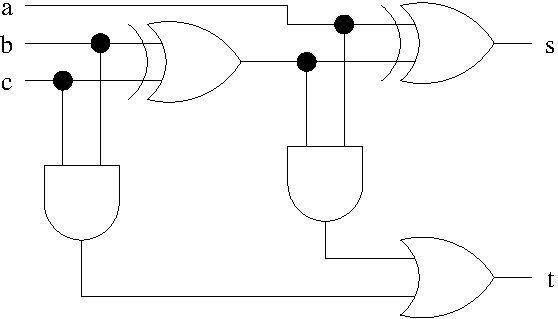
\includegraphics[width=6cm]{add3.pdf}$$

\paragraph{Questions :} 

\begin{question}[«~circuit logique~» : combinatoire]
Combien y a-t-il de combinaisons différentes possibles en entrée du circuit logique considéré 
(nombre de triplets $(a,b,c)$ différents) ?
\end{question}

\begin{question}[«~circuit logique~» : table de vérité]
Déterminer les valeurs des sorties $(s,t)$ pour chaque triplet d'entrée $(a,b,c)$ possible.
\end{question}

Dans la pratique, un circuit logique est conçu pour une fonction précise.
Il faut alors vérifier qu'il remplit bien sa fonction.
\begin{question}[«~circuit logique~» : vérification]
Vérifier que ce circuit effectue l'addition des 3 bits 
$a$, $b$ et $c$ : $s$ est la somme et $t$ la retenue.

\begin{tabular}{lr}
    & $a$ \\
$+$ & $b$ \\
$+$ & $c$ \\
\hline
$=$ & $t\ s$
\end{tabular}
\end{question}

%-------------------------------------------------------------------------
\newpage
\subsection{Généralisation}
%-------------------------------------------------------------------------
Les 3 opérateurs booléens de base :
\texttt{not} (négation), \texttt{and} (conjonction) et 
\texttt{or} (disjonction), sont définis par leur table de vérité.

$$\begin{tabular}{|c|c|c|}
\hline
\makebox[3cm]{négation} & \makebox[3cm]{disjonction} & \makebox[3cm]{conjonction} \\
$\overline{a}$ & $a+b$ & $a \cdot b$\\
\hline
\tt not a & \tt a or b & \tt a and b\\
$\begin{array}[t]{|c|c|}
\hline
a & {\overline{a}}\\
\hline
0 & 1\\
1 & 0\\
\hline
\end{array}$ &
$\begin{array}[t]{|c|c|c|}
\hline
a & b & {a+b}\\
\hline
0 & 0 & 0\\
0 & 1 & 1\\
1 & 0 & 1\\
1 & 1 & 1\\
\hline
\end{array}$ &
$\begin{array}[t]{|c|c|c|}
\hline
a & b & {a\cdot b}\\
\hline
0 & 0 & 0\\
0 & 1 & 0\\
1 & 0 & 0\\
1 & 1 & 1\\
\hline
\end{array}$ \\[2.7cm]
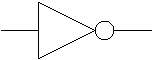
\includegraphics[height=0.75cm]{non.pdf} & 
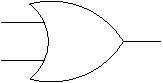
\includegraphics[height=0.75cm]{ou.pdf}  &
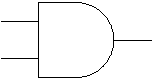
\includegraphics[height=0.75cm]{et.pdf}  \\
\hline
 & \tt not (a or b) & \tt not (a and b) \\[0.3cm]
 & 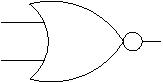
\includegraphics[height=0.75cm]{nonOu.pdf} & 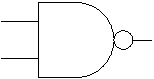
\includegraphics[height=0.75cm]{nonEt.pdf}\\
\hline
\end{tabular}$$

\noindent On peut démontrer que ces opérateurs vérifient les propriétés suivantes :
$$\begin{tabular}{l@{ : }ll}
\multicolumn{3}{l}{$\forall a, b, c \in \{0;1\}$}\\
identité        & $a = \overline{\overline{a}}$ \\
élément neutre  & $a + 0 = a$ & $a \cdot 1 = a$ \\
élément nul     & $a + 1 = 1$ & $a \cdot 0 = 0$ \\
idempotence     & $a + a = a$ & $a \cdot a = a$ \\
complémentarité & $a + \overline{a} = 1$ & $a \cdot \overline{a} = 0$ \\
absorption      & $a + (a \cdot b) = a$ & $a \cdot (a + b) = a$ \\
simplification  & $a + (\overline{a} \cdot b) = (a + b) $ & $a \cdot (\overline{a} + b) = (a \cdot b)$ \\
commutativité   & $(a+b) = (b+a)$ & $(a \cdot b) = (b \cdot a)$\\
associativité   & $(a+b)+c = a+(b+c)$ & $(a\cdot b)\cdot c = a\cdot (b\cdot c)$ \\
distributivité  & $a + (b \cdot c) = (a+b) \cdot (a+c)$ & $a \cdot (b+ c) = (a \cdot b)+(a\cdot c)$ \\
De Morgan       & $\overline{a + b} = \overline{a} \cdot \overline{b}$
                & $\overline{a\cdot b} = \overline{a} + \overline{b}$
\end{tabular}$$

\begin{question}[opérateurs booléens : distributivité]
Démontrer les propriétés de distributivité :\\ $\forall a, b, c \in \{0;1\}$
\begin{enumerate}
\item $a + (b \cdot c) = (a+b) \cdot (a+c)$
\item $a \cdot (b + c) = (a \cdot b)+(a\cdot c)$
\end{enumerate}
On comparera pour cela les tables de vérité des deux membres de l'égalité.
\end{question}

\begin{question}[opérateurs booléens : De Morgan]
Démontrer les propriétés de De Morgan :\\ $\forall a, b \in \{0;1\}$
\begin{enumerate}
\item $\overline{a + b} = \overline{a} \cdot \overline{b}$
\item $\overline{a\cdot b} = \overline{a} + \overline{b}$
\end{enumerate}
On comparera pour cela les tables de vérité des deux membres de l'égalité.
\end{question}


A partir de ces 3 opérateurs de base, on peut définir des opérateurs dérivés tels que l'équiva\-lence ($\Leftrightarrow$), l'implication ($\Rightarrow$) et la disjonction exclusive ($\oplus$).
$$\begin{tabular}{|c|c|c|}
\hline
\makebox[3cm]{équivalence} & \makebox[3cm]{implication} & \makebox[3cm]{ou exclusif} \\
$a \Leftrightarrow b$ & $a \Rightarrow b$ & $a \oplus b$\\
\hline
\tt a == b & & \tt a != b \\
$\begin{array}[t]{|c|c|c|}
\hline
a & b & {a \Leftrightarrow b}\\
\hline
0 & 0 & 1\\
0 & 1 & 0\\
1 & 0 & 0\\
1 & 1 & 1\\
\hline
\end{array}$ &
$\begin{array}[t]{|c|c|c|}
\hline
a & b & {a \Rightarrow b}\\
\hline
0 & 0 & 1\\
0 & 1 & 1\\
1 & 0 & 0\\
1 & 1 & 1\\
\hline
\end{array}$ &
$\begin{array}[t]{|c|c|c|}
\hline
a & b & {a \oplus b}\\
\hline
0 & 0 & 0\\
0 & 1 & 1\\
1 & 0 & 1\\
1 & 1 & 0\\
\hline
\end{array}$ \\[2.7cm]
 & & 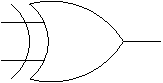
\includegraphics[height=0.75cm]{xor.pdf}  \\
%$\overline{(a + b)} + (a \cdot b)$ & $\overline{a} + b$ & $(a + b) \cdot \overline{(a \cdot b)}$ \\
% & & $a \cdot \overline{b} + \overline{a} \cdot b$\\
\hline
\end{tabular}$$

\begin{question}[opérateurs booléens : opérateurs dérivés]
Définir l'équivalence ($\Leftrightarrow$), l'implication ($\Rightarrow$) et la disjonction exclusive ($\oplus$)
en fonction des 3 opérateurs de base (négation, conjonction et disjonction).
\end{question}


%-------------------------------------------------------------------------
\subsection{Applications}
%-------------------------------------------------------------------------

\begin{question}[développer une expression booléenne]
Développer les expressions booléennes suivantes
en justifiant chaque étape du développement.
Vérifier avec \python.
\begin{enumerate}  
\item $t = \overline{a + b + \overline{c} \cdot \overline{d}}$
\item $t = \overline{a \cdot \overline{b} \cdot c \cdot d}$ 
\item $t = \overline{a \cdot \overline{b} \cdot {c} + \overline{d}}$
\item $t = \overline{\overline{a} \cdot \overline{b} + {c} \cdot {d}}$
\item $t = \overline{a + b \cdot c \cdot d}$
\item $t = \overline{\overline{a} \cdot b + {c} + \overline{d}}$
\end{enumerate}
\end{question}

\begin{question}[fonctions booléennes binaires]
Combien peut-on définir de fonctions booléennes binaires $f_i$ :
$\forall a, b, c \in \{0;1\}, c = f_i(a,b)$ ? Identifier chacune de ces fonctions :
on doit en particulier retrouver les opérateurs de base $\cdot$ et $+$.
\end{question}
%-------------------------------------------------------------------------
%\newpage
\subsection{Entraînement}
%-------------------------------------------------------------------------

%-------------------------------------------------------------------------
\subsubsection{Enoncé}
%-------------------------------------------------------------------------


\paragraph{Objectif :} établir la table de vérité d'une expression booléenne.

\paragraph{Méthode :} introduire des variables intermédiaires pour faciliter les calculs.

\paragraph{Vérification :} vérifier avec \python{} les résultats obtenus pour 
différentes valeurs des entrées.

%-------------------------------------------------------------------------
\newpage
\subsubsection{Exemple}
%-------------------------------------------------------------------------
Soit à établir la table de vérité de l'expression :
$z = ((\overline{a} \Rightarrow \overline{b}) \cdot (b \Rightarrow c)) \Rightarrow (({c} \Rightarrow {a}) \Rightarrow d)$

\paragraph{Méthode :}
On pose : $p = (\overline{a} \Rightarrow \overline{b})$, $q = (b \Rightarrow c)$, $r = p\cdot q$,
$s = ({c} \Rightarrow {a})$ et $t = (s \Rightarrow d)$. On a donc finalement : $z = (r \Rightarrow t)$.

Puis, on transforme les expression du type ($p \Rightarrow q$) en ($\overline{p}+q$); 
elles ont en effet les mêmes tables de vérité :\\
\centerline{$\begin{array}[t]{|c|c|c|}
\hline
p & q & {p \Rightarrow q}\\
\hline
0 & 0 & 1\\
0 & 1 & 1\\
1 & 0 & 0\\
1 & 1 & 1\\
\hline
\end{array}
\hspace*{1cm}
\begin{array}[t]{|c|c|c|c|}
\hline
p & \overline{p} & q & {\overline{p} + q}\\
\hline
0 & 1 & 0 & 1\\
0 & 1 & 1 & 1\\
1 & 0 & 0 & 0\\
1 & 0 & 1 & 1\\
\hline
\end{array}$}

\paragraph{Résultat :}
La table de vérité recherchée comporte $2^4 = 16$ entrées (4 variables $a$, $b$, $c$, $d$, 
de 2 valeurs possibles chacune : $0$ ou $1$) :

$$\begin{array}{|c|c|c|c||c|c|c|c|c||c|}
\hline
a & b & c & d & p & q & r & s & t & z \\
  &   &   &   & 
  \overline{a} \Rightarrow \overline{b} &
  b \Rightarrow c &
  p \cdot q &
  c \Rightarrow a &
  s \Rightarrow d &
  r \Rightarrow t \\
  &   &   &   &
  a + \overline{b} &
  \overline{b} + c &
                   &
  \overline{c} + a &
  \overline{s} + d &
  \overline{r} + t \\
\hline
0 & 0 & 0 & 0 & 1 & 1 & 1 & 1 & 0 & 0 \\
0 & 0 & 0 & 1 & 1 & 1 & 1 & 1 & 1 & 1 \\
0 & 0 & 1 & 0 & 1 & 1 & 1 & 0 & 1 & 1 \\
0 & 0 & 1 & 1 & 1 & 1 & 1 & 0 & 1 & 1 \\
0 & 1 & 0 & 0 & 0 & 0 & 0 & 1 & 0 & 1 \\
0 & 1 & 0 & 1 & 0 & 0 & 0 & 1 & 1 & 1 \\
0 & 1 & 1 & 0 & 0 & 1 & 0 & 0 & 1 & 1 \\
0 & 1 & 1 & 1 & 0 & 1 & 0 & 0 & 1 & 1 \\
1 & 0 & 0 & 0 & 1 & 1 & 1 & 1 & 0 & 0 \\
1 & 0 & 0 & 1 & 1 & 1 & 1 & 1 & 1 & 1 \\
1 & 0 & 1 & 0 & 1 & 1 & 1 & 1 & 0 & 0 \\
1 & 0 & 1 & 1 & 1 & 1 & 1 & 1 & 1 & 1 \\
1 & 1 & 0 & 0 & 1 & 0 & 0 & 1 & 0 & 1 \\
1 & 1 & 0 & 1 & 1 & 0 & 0 & 1 & 1 & 1 \\
1 & 1 & 1 & 0 & 1 & 1 & 1 & 1 & 0 & 0 \\
1 & 1 & 1 & 1 & 1 & 1 & 1 & 1 & 1 & 1 \\
\hline
\end{array}$$

%\newpage
\paragraph{Vérification :} On peut vérifier le résultat obtenu
avec \python{} en utilisant les mêmes notations que précédemment.

L'expression $z$ est simplement calculée par la séquence d'affectations suivante :
\vspace*{2mm}

\begin{minipage}{4cm}
\begin{Verbatim}[frame=single]
 p = a or not b
 q = not b or c
 r = p and q
 s = not c or a
 t = not s or d
 z = not r or t
\end{Verbatim}
\end{minipage}
\hfill
\begin{minipage}{5cm}\footnotesize
\begin{Verbatim}
>>> a, b, c, d = 0, 0, 0, 0
>>> p = a or not b
>>> q = not b or c
>>> r = p and q
>>> s = not c or a
>>> t = not s or d
>>> z = not r or t
>>> z
0
\end{Verbatim}
\end{minipage}
\hfill
\begin{minipage}{5cm}\footnotesize
\begin{Verbatim}
>>> a, b, c, d = 0, 1, 0, 1
>>> p = a or not b
>>> q = not b or c
>>> r = p and q
>>> s = not c or a
>>> t = not s or d
>>> z = not r or t
>>> z
1
\end{Verbatim}
\end{minipage}

\newpage
L'utilisation des boucles en \python{} permettra d'obtenir directement la table de vérité.

\noindent
\begin{minipage}[t]{10cm}\footnotesize
\begin{lstlisting}
print("a","b","c","d","|",\
      "p","q","r","s","t","|","z")
print(7*"-","|",9*"-","|",1*"-")
for a in [0,1] :
    for b in [0,1] :
        for c in [0,1] :
            for d in [0,1] :
                p = a or not b
                q = not b or c
                r = p and q
                s = not c or a
                t = not s or d
                z = not r or t
                print(a,b,c,d,"|", \
                      int(p),int(q),int(r),\
                      int(s),int(t),"|",\
                      int(z))
\end{lstlisting}
\end{minipage}
\hfill
\begin{minipage}[t]{4cm}\footnotesize
\begin{Verbatim}
a b c d | p q r s t | z
------- | --------- | -
0 0 0 0 | 1 1 1 1 0 | 0
0 0 0 1 | 1 1 1 1 1 | 1
0 0 1 0 | 1 1 1 0 1 | 1
0 0 1 1 | 1 1 1 0 1 | 1
0 1 0 0 | 0 0 0 1 0 | 1
0 1 0 1 | 0 0 0 1 1 | 1
0 1 1 0 | 0 1 0 0 1 | 1
0 1 1 1 | 0 1 0 0 1 | 1
1 0 0 0 | 1 1 1 1 0 | 0
1 0 0 1 | 1 1 1 1 1 | 1
1 0 1 0 | 1 1 1 1 0 | 0
1 0 1 1 | 1 1 1 1 1 | 1
1 1 0 0 | 1 0 0 1 0 | 1
1 1 0 1 | 1 0 0 1 1 | 1
1 1 1 0 | 1 1 1 1 0 | 0
1 1 1 1 | 1 1 1 1 1 | 1
\end{Verbatim}
\end{minipage}


%-------------------------------------------------------------------------
%\newpage
\subsubsection{Questions}
%-------------------------------------------------------------------------

Etablir la table de vérité des expressions booléennes suivantes en faisant apparaître des variables intermédiaires de calcul.

\noindent\begin{minipage}[t]{7cm}
\begin{enumerate}  
\item $z = ((a \Rightarrow b) \cdot (b \Rightarrow \overline{c})) \Rightarrow (\overline{c} \Rightarrow \overline{a})$
\item $z = ((\overline{a} \Rightarrow \overline{b}) \cdot (b \Rightarrow c)) \Rightarrow ({c} \Rightarrow {a})$
\item $z = ((a \cdot b) \Rightarrow (b \cdot c)) \Rightarrow ({c} + \overline{a})$
\item $z = ((a + b) \Rightarrow (b + c)) \Rightarrow (\overline{c} \Rightarrow \overline{a})$
\item $z = ((a \Rightarrow b) + (b \Rightarrow c)) \Rightarrow (\overline{c} + \overline{a})$
\item $z = ((a \Rightarrow b) + (b \Rightarrow c)) \Rightarrow (\overline{c} \Rightarrow \overline{a})$
\item $z = ((a \Rightarrow b) \cdot (b \Rightarrow \overline{c})) \Rightarrow (\overline{c} \oplus \overline{a})$
\item $z = ((\overline{a} \Rightarrow \overline{b}) \cdot (b \Rightarrow c)) \oplus ({c} \Rightarrow {a})$
\item $z = ((a \cdot b) \oplus (b \cdot c)) \Rightarrow ({c} + \overline{a})$
\item $z = ((a \oplus b) \Rightarrow (b + c)) \Rightarrow (\overline{c} \oplus \overline{a})$
\item $z = ((a \Rightarrow b) + \overline{(b \Rightarrow c)}) \Rightarrow (\overline{c} + \overline{a})$ 
\item $z = ((a \Rightarrow b) + (b \oplus c)) \Rightarrow (\overline{c} \Rightarrow \overline{a})$
%\item $z = ((a \Rightarrow b) + (b \Rightarrow \overline{c})) \Rightarrow (\overline{c} \oplus \overline{a})$
%\item $z = ((\overline{a} \Rightarrow \overline{b}) + (b \Rightarrow c)) \oplus ({c} \Rightarrow {a})$
%\item $z = ((a + b) \oplus (b \cdot c)) \Rightarrow ({c} + \overline{a})$
%\item $z = ((a \oplus b) \Rightarrow (b \cdot c)) \Rightarrow (\overline{c} \oplus \overline{a})$
%\item $z = ((a \Rightarrow b) \cdot \overline{(b \Rightarrow c)}) \Rightarrow (\overline{c} + \overline{a})$ 
%\item $z = ((a \Rightarrow b) \cdot (b \oplus c)) \Rightarrow (\overline{c} \Rightarrow \overline{a})$
\end{enumerate}
\end{minipage}
\hfill
\begin{minipage}[t]{7cm}
\begin{enumerate}\setcounter{enumi}{12}
%\item $z = (\overline{(a \Rightarrow b)} + (b \Rightarrow \overline{c})) \Rightarrow (\overline{c} \oplus \overline{a})$
%\item $z = ((\overline{a} \Rightarrow {b}) + (b \Rightarrow c)) \oplus ({c} \Rightarrow {a})$ 
%\item $z = (\overline{(a + b)} \oplus (b \cdot c)) \Rightarrow ({c} + \overline{a})$ 
%\item $z = (\overline{(a \oplus b)} \Rightarrow (b \cdot c)) \Rightarrow (\overline{c} \oplus \overline{a})$ 
%\item $z = ((a \Rightarrow b) \cdot \overline{(b \Rightarrow c)}) \Rightarrow ({c} + {a})$ 
%\item $z = ((a \Rightarrow b) \cdot (b \oplus c)) \Rightarrow \overline{(\overline{c} \Rightarrow \overline{a})}$ 
\item $z = ({(a \Rightarrow b)} + \overline{(b \Rightarrow \overline{c})}) \Rightarrow (\overline{c} \oplus \overline{a})$ 
\item $z = (({a} \Rightarrow {b}) + \overline{(b \Rightarrow c)}) \oplus ({c} \Rightarrow {a})$
\item $z = ({(a + b)} \oplus \overline{(b \cdot c)}) \Rightarrow ({c} + \overline{a})$
\item $z = (\overline{(a \oplus \overline{b})} \Rightarrow (b \cdot c)) \Rightarrow (\overline{c} \oplus \overline{a})$
\item $z = ((a \Rightarrow \overline{b}) \cdot \overline{(b \Rightarrow c)}) \Rightarrow ({c} + {a})$
\item $z = ((a \Rightarrow \overline{b}) \cdot (b \oplus c)) \Rightarrow \overline{(\overline{c} \Rightarrow \overline{a})}$
\item $z = ({(a \Rightarrow b)} \cdot \overline{(b \Rightarrow \overline{c})}) \Rightarrow (\overline{c} \oplus \overline{a})$ 
\item $z = (({a} \Rightarrow {b}) \cdot \overline{(b \Rightarrow c)}) \oplus ({c} \Rightarrow {a})$
\item $z = ({(a + b)} + \overline{(b \cdot c)}) \Rightarrow ({c} + \overline{a})$
\item $z = (\overline{(a \oplus \overline{b})} \Rightarrow (b \cdot c)) \Rightarrow (\overline{c} \oplus \overline{a})$
\item $z = ((a \Rightarrow \overline{b}) \cdot \overline{(b \Rightarrow c)}) \Rightarrow ({c} \cdot {a})$
\item $z = ((a \Rightarrow \overline{b}) \cdot (b + c)) \Rightarrow \overline{(\overline{c} \Rightarrow \overline{a})}$
\end{enumerate}
\end{minipage}

%-------------------------------------------------------------------------
\subsection{Révisions}
%-------------------------------------------------------------------------

$$\begin{tabular}{|ll@{ : }l|}
\hline
\textbf{Cours} & \cite{cours} & chapitre 2, section 2.3.1 \\
\textbf{TD}    & \cite{td}    & exercices 2.5 à 2.7, 2.29 \\
\hline
\end{tabular}$$
